\documentclass{beamer}

\usetheme{zg}

\graphicspath{{./fig/}}

\title{Exemplo de Apresentação}
\date{\today}
\author{Fernando Camargo}
\institute{ZG Soluções}


\begin{document}
\maketitle

\section{Slides básicos}

\begin{frame}{O Problema do Planejamento Energético de Sistemas\\Hidrotérmicos}
  
  Considerações:
  \begin{outline}
    \1<1-> Decisões de operação afetam decisões futuras: reservatórios
    \1<2-> Acoplamento de usinas na mesma bacia
    \1<3-> Aleatoriedade das vazões
    \1<4-> Objetivos:
      \2<4-> Minimizar custo de produção (custo térmico)
      \2<5-> Aumentar produção hidrelétrica para diminuir termelétrica
      \2<6-> Definir uma estratégia de geração para cada usina de interconectada
      \2<7-> Atender demanda com confiabilidade
  \end{outline}
\end{frame}

\begin{frame}{O Problema do Planejamento Energético de Sistemas\\Hidrotérmicos}
  
  Características:
  \begin{outline}
    \1<1-> Problema dinâmico de otimização envolvendo o tempo
    \1<2-> Problema não separável
    \1<3-> Função de objetivo não linear e não convexa
    \1<4-> Problema estocástico
    \1<5-> De grande porte
  \end{outline}
  \onslide<6->{Adoção de único modelo inviável.}\\
  \onslide<7->{\alert{Solução: decomposição do problema.}}
\end{frame}

\begin{frame}{Algoritmos utilizados}
  
  \begin{outline}
  \0 \onslide<1->{Algoritmos:}
    \1<1-> Programa Dinâmica e Estocástica
      \2 Uma tabela de soluções ótimas para cada estado do sistema é gerada
      \2 Explosão combinatorial de estados
      \2 Tentativas de simplificação do problema uso dessa técnica
    \1<2-> Técnicas não lineares baseadas na teoria lagrangeana
    \1<2-> Técnicas não lineares por fluxos de redes
  \0 \onslide<3->{Problemas:}
    \1<3-> Não garantia de ótimo global
    \1<4-> Problemas de convergência 
    \1<5-> Computabilidade
  \end{outline}
\end{frame}

\section{Tabelas e Figuras}

\begin{frame}{Matriz energética brasileira}
  A Tabela \ref{table:dependenciaNatureza2012} de \cite{junior1998} mostra como a atual matriz brasileira de produção de energia elétrica é muito dependente dos fluxos da Natureza.
  
  \begin{table}
  \caption{Dependência da Natureza para geração de energia elétrica (Fonte: ANEEL (2012))}
  \label{table:dependenciaNatureza2012}
  \begin{tabular}{|l|l|l|l|}
      \hline
      Hidro       & 84.094,7   & Térmica      & 32.730,8  \\ \hline
      Eólica      & 1.820,3    & Nuclear      & 2.007,0    \\ \hline
      Total       & 85.915     & Total        & 34.737,8  \\ \hline
      \% do total & 71,2\%     & \% do total  & 28,8\%    \\ \hline
  \end{tabular}
  \end{table}
\end{frame}

\begin{frame}{Principais componentes de uma Usina Hidrelétrica}
  
  \begin{figure}
    \centering
    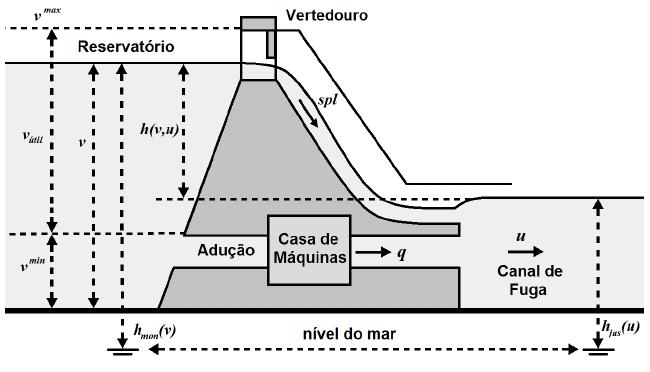
\includegraphics[width=\textwidth]{./fig/Componentes-usinas-hidreletricas.jpg}
    \label{fig:componentesUsinasHidreletricas}
  \end{figure}
\end{frame}

\section{Algoritmos}

% PDF com comandos em português: http://www.cs.toronto.edu/~frank/Useful/algorithm2e.pdf
% Item 9.3, pág. 24
\begin{frame}{Pseudocódigo}
  \begin{algorithm2e}[H]
    \DontPrintSemicolon
    \LinesNumbered
    \SetAlgoLined
    \BlankLine
    \Saida{melhor solução encontrada ao fim da execução}
    \BlankLine
    INICIALIZE população com soluções candidatas aleatórias\;
    AVALIE cada candidato\;
    \Enqto{CONDIÇÃO DE TÉRMINO não é satisfeita}{
      SELECIONE pais\;
      RECOMBINE pares de pais\;
      REALIZE MUTAÇÃO dos filhos obtidos\;
      AVALIE os novos candidatos\;
      SELECIONE indivíduos para a próxima geração\;
    }
  \caption{Pseudocódigo de Algoritmos Evolucionários \label {alg:pseudocodigoAlgoritmosEvolucionarios}}
  \end{algorithm2e}
\end{frame}

% Documentação do Minted: https://github.com/gpoore/minted/blob/master/source/minted.pdf
\begin{frame}[fragile]{Código Interno}
  \begin{minted}[linenos, % Número nas linhas
    fontsize=\tiny]{java}
    public class HelloWorld {

	public static void main(String[] args) {
	    // Prints "Hello, World" to the terminal window.
	    System.out.println("Hello, World");
	}

    }
  \end{minted}
\end{frame}

\begin{frame}[fragile]{Código Externo}
  \inputminted[fontsize=\tiny]{groovy}{cod/Periodo.groovy}
\end{frame}


\section{Ambientes Matemáticos}

\begin{frame}{O que são números primos?}
  \begin{definition}
    Um \alert{número primo} é um número que possui exatamente dois divisores.
  \end{definition}
  \begin{example}
    \begin{itemize}
    \item 2 é primo (dois divisores: 1 e 2).
    \item 3 é primo (dois dividores: 1 e 3).
    \item 4 não é primo (\alert{três} divisores: 1, 2, e 4).
    \end{itemize}
  \end{example}
\end{frame}

\begin{frame}{Não existe o maior número primo}
  \begin{theorem}
    Não existe o maior número primo.
  \end{theorem}
  \begin{proof}
    \begin{enumerate}
      \item Suponha que $p$ fosse o maior número primo.
      \item Seja $q$ o produto dos primeiros $p$ números.
      \item Então $q + 1$ não é divisível por nenhum deles.
      \item Mas $q + 1$ é maior que $1$, portanto divisível por algum número primo não existente nos primeiros $p$ números.\qedhere
    \end{enumerate}
  \end{proof}
  \uncover<2->{A prova usa \textit{reductio ad absurdum}.}
\end{frame}

\section{Referências}

\begin{frame}[allowframebreaks]{Referências}
  %\nocite{*} % Se quiser que todas citações apareçam
  \bibliography{./bib/exemplo.bib}
\end{frame}

\end{document}
